\subsection{Combining Parameter}

Thus far, we have not seen type B regions, that are not caused by overlapping type A regions.
We now want to change multiple parameters at the same time to imitate the function of the original model better.
For this, we introduce new parameters, $p_x$ and $p_y$, and define the actual model parameters dependent on those two.

\subsubsection{Defining $a_R = 1 + p_x$, $b_R = 2 \cdot px$, and $c_L = p_y$}

\todo{better imitation but nothing was found}

\subsubsection{Defining $a_R = 1 + 2 \cdot p_x$, $b_R = px$, and $c_L = p_y$}

This definition of $a_R$ and $b_R$ is similar to before, but now $p_x$ has double the effect on $a_R$ and half the effect on $b_R$.
It was created by accident since it does not imitate the original model as nicely as before.
\Cref{fig:quadratic.full.2aR1bR_cL.2d.full} shows the 2D scan of the different periods.
Regions we will have a closer look at, are marked with red rectangles.

\begin{figure}
    \centering
    \includegraphics[width=0.6\textwidth]{21_002_Quadratic_2aR1bR_cL/2D_Period_Selected/result.png}
    \caption{2D Scan of Periods of Quadratic Model with ...}
    \label{fig:quadratic.full.2aR1bR_cL.2d.full}
\end{figure}

The first enhanced region, shown in \Cref{fig:quadratic.full.2aR1bR_cL.2d.1}, has two areas with stable cycles of period 6 that overlap.
\Cref{fig:quadratic.regions.2aR1bR_cL.2d.1} shows the borders of the two regions.
It was created by halving the model and scanning for the borders of regions of different periods.
We will see that the bottom area is a type B area, and therefore the period in the halved model is double the period in the full model.

\begin{figure}
    \centering
    \begin{subfigure}{0.4\textwidth}
        \centering
        \includegraphics[width=\textwidth]{21_002_Quadratic_2aR1bR_cL/P6/2D_Period_P6/result.png}
        \caption{Periods}
        \label{fig:quadratic.full.2aR1bR_cL.2d.1}
    \end{subfigure}
    \begin{subfigure}{0.4\textwidth}
        \centering
        \includegraphics[width=\textwidth]{21_002_Quadratic_2aR1bR_cL/P6/2D_Regions_P6/result.png}
        \caption{Period Regions}
        \label{fig:quadratic.regions.2aR1bR_cL.2d.1}
    \end{subfigure}
    \caption{2D Scans of First Marked Region}
\end{figure}

\todo{cobwebs A und B}
